%%%%%%%%%%%%%%%%%%%%%%%%%%%%%%%%%%%%%%%%%%%%%%%%%%%%%%%%%%%%%%%%%%%%%%%%%%%
%
% Template for a LaTex article in English.
%
%%%%%%%%%%%%%%%%%%%%%%%%%%%%%%%%%%%%%%%%%%%%%%%%%%%%%%%%%%%%%%%%%%%%%%%%%%%

\documentclass{article}

% AMS packages:
\usepackage{amsmath, amsthm, amsfonts}
\usepackage{algorithm}
\usepackage[hyperref, UTF8]{ctex}
\usepackage[noend]{algpseudocode}
\usepackage{graphicx}
\usepackage{subcaption}
\usepackage[top=0.8in, bottom=0.8in, left=1in, right=1in]{geometry}
\graphicspath{ {images/} }

% Theorems
%-----------------------------------------------------------------
\newtheorem{thm}{Theorem}[section]
\newtheorem{cor}[thm]{Corollary}
\newtheorem{lem}[thm]{Lemma}
\newtheorem{prop}[thm]{Proposition}
\theoremstyle{definition}
\newtheorem{defn}[thm]{Definition}
\theoremstyle{remark}
\newtheorem{rem}[thm]{Remark}

\makeatletter
\def\BState{\State\hskip-\ALG@thistlm}
\makeatother
%\newcommand*{\rom}[1]{\expandafter\@slowromancap\romannumeral #1@}
\newcommand{\rom}[1]{\uppercase\expandafter{\romannumeral #1\relax}}
% Shortcuts.
% One can define new commands to shorten frequently used
% constructions. As an example, this defines the R and Z used
% for the real and integer numbers.
%-----------------------------------------------------------------
\def\RR{\mathbb{R}}
\def\ZZ{\mathbb{Z}}

% Similarly, one can define commands that take arguments. In this
% example we define a command for the absolute value.
% -----------------------------------------------------------------
\newcommand{\abs}[1]{\left\vert#1\right\vert}

% Operators
% New operators must defined as such to have them typeset
% correctly. As an example we define the Jacobian:
% -----------------------------------------------------------------
\DeclareMathOperator{\Jac}{Jac}

%-----------------------------------------------------------------
\title{Report of paper (Isotopic Approximation within a Tolerance Volume)}
\author{张胜威\\
  %% \small Dept. Templates and Editors\\
  %% \small E12345\\
  %% \small Spain
}

\begin{document}
\maketitle

%% \abstract{Compiling Embedded\_thin\_shell progress}
\section{Target}
For a surface $\mathbb{S}$, we construct a tolerance volume $\Omega$ which is a topological thickening of a surface $\mathbb{S}$. Our goal is to generate as output a surface triangle mesh located within $\Omega$, isotopic to the boundary components of $\Omega$, and with a low triangle count.
\section{Algorithm Overview}
Figure 1 depicts the three main steps of our approach:
\begin{figure}[H]
 	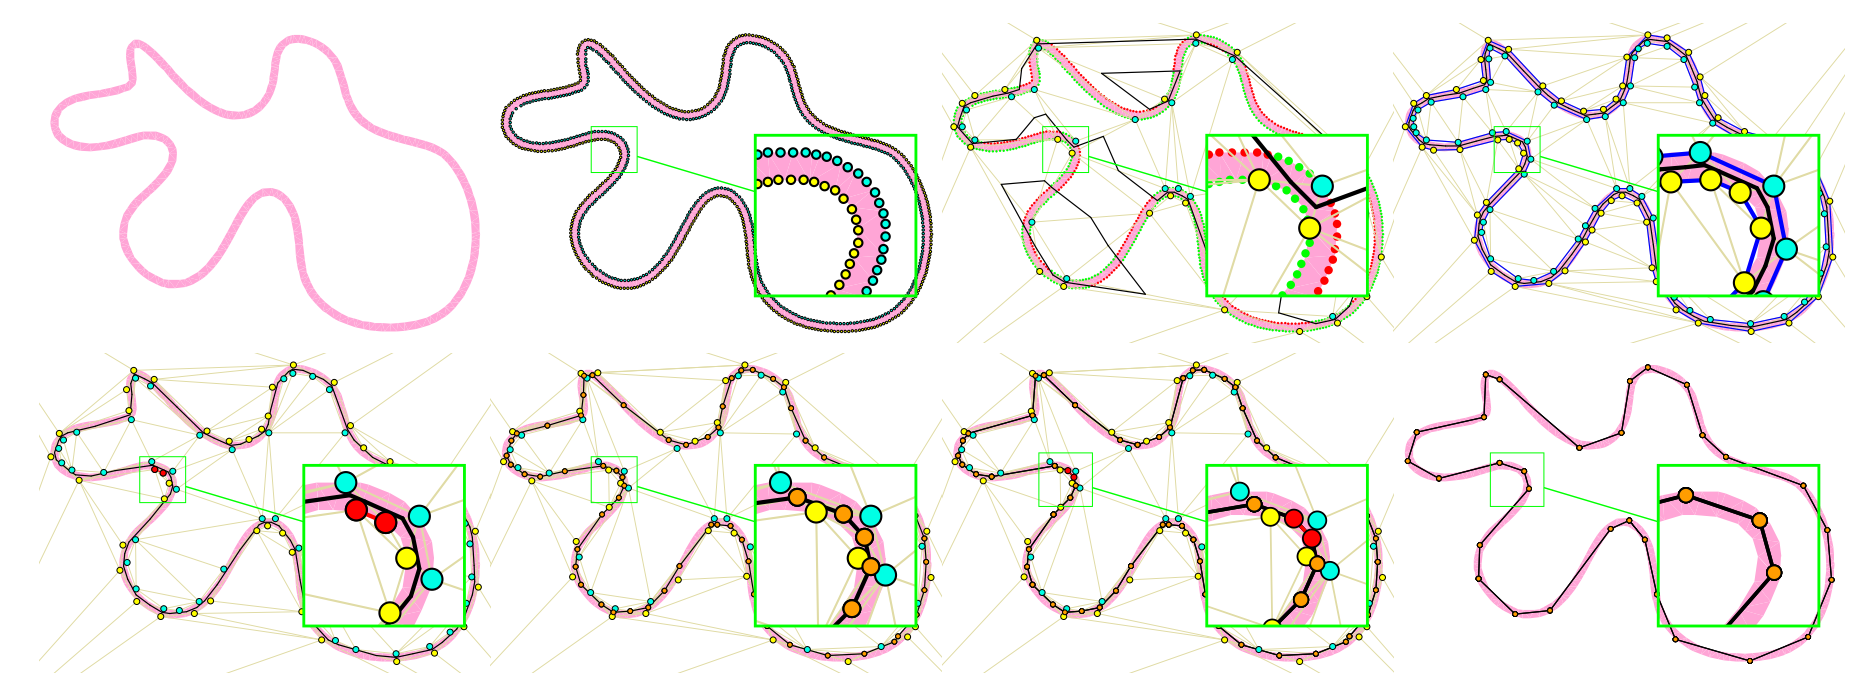
\includegraphics[width=16cm]{1}
	\caption[Overview]
 	{Overview of our algorithm. Top: input tolerance $\Omega$, sampling of $\partial \Omega$, mesh refinement by inserting a subset of the sample points, and topology condition met. Samples that are well classified are depicted in green, and in red otherwise. The boundary of the simplicial tolerance volume $\partial \Gamma$ is depicted with blue edges. Bottom: simplification of $\partial \Gamma$, mutual tessellation of zero-set, simplification of zero-set, and final output.}
 	\centering
\end{figure}
\begin{description}
  \item[1.] Generates a dense point sample S on the boundary of the tolerance volume $\partial \Omega$.
  \item[2.] Refine, select points from $\partial \Omega$ to construct $\Gamma$ -- a approximation of volume $\Omega$, By adding points to the triangulation $\tau$, meanwhile, maintaining a piecewise-linear function $f(\mathtt{s})$ interpolated on that triangulation.
  \item[3.] Simplification, Simplify the zero point set $\mathcal{Z}$ of the piecewise-linear function(the final output), By do on $\tau$ edge collapse in $\partial \Gamma$, perform mutual tessellation between $\mathcal{Z}$ and $\partial \Gamma$, then do edge collapse of all edges again.
\end{description}

\section{Construct the $\Omega$ from a input Surface $\mathbb{S}$}
Paper did not elaborate.
\section{Refinement}
\subsection{Initialization}
Construct an initial 3D Delaunay triangulation ($\tau$) with the eight corners of a loose bounding box of $\mathtt{S}$ (with the same function value as outer boundary),  and maintaining a piecewise-linear function $f(\mathtt{s})$ interpolated on the triangulation, and the error function $\epsilon(\mathtt{s})$:
\begin{equation}
  \begin{array}{l}
f(\mathtt{s}) \approx \left\{
\begin{array}{lcl}
{+1} &\text{if} & s \in \partial \Omega_1 \text{ outer boundary} \\
{-1} &\text{if} & s \in \partial \Omega_2 \text{ inner boundary} \\  
\end{array}  
\right.\\
\epsilon(\mathtt{s}) = \left\{
\begin{array}{lcl}
{\parallel f(\mathtt{s})-1 \parallel} &\text{if} & s \in \partial \Omega_1 \text{ outer boundary} \\
{\parallel f(\mathtt{s})+1 \parallel} &\text{if} & s \in \partial \Omega_2 \text{ inner boundary} \\  
\end{array}  
\right.\\
\end{array}
\end{equation}
Here we define midpoints on the edges between $\partial \Omega_1$ and $\partial \Omega_2$, as zero-points $\mathcal{Z}$. Our refinement of $\tau$ end up with the function $f(\mathtt{s})$ can well classify $\mathtt{S}$ from $\partial \Omega_1$ between $\partial \Omega_2$. Figure 2 illustrates in 2D a refinment of $\tau$, the zero-set $\mathcal{Z}$ and the classification of $\mathtt{S}$.
\begin{figure}[H]
 	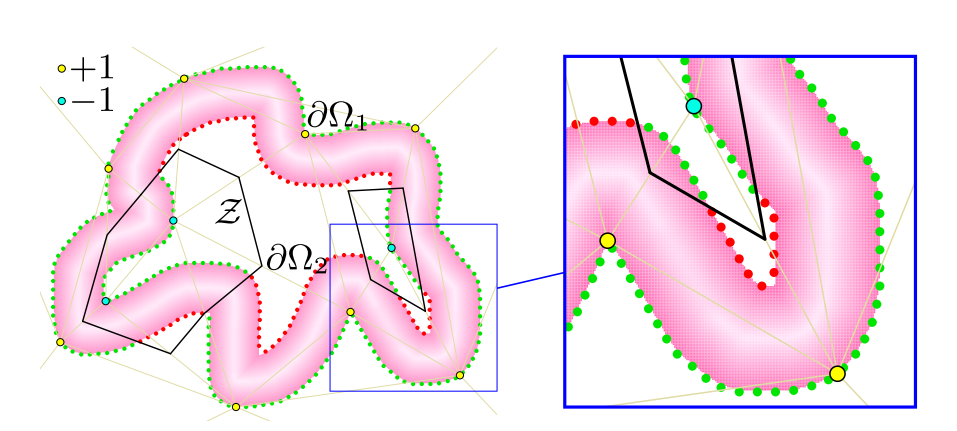
\includegraphics[width=12cm]{2}
	\caption[Classification of $\mathcal{S}$]
        {Classification of S. The black solid edges depict the zero-set Z of f. A sample classified as good is depicted in green, and in red otherwise.}
 	\centering
\end{figure}
\subsection{Procedure}
Our goal is to construct a $\Gamma$ approximate $\Omega$. We get it by insert one sample point at a time into $\tau$ and update the Delaunay property, until $\mathcal{Z}$ classifies all samples of  $\mathtt{S}$ as good, or equivalently, until $\mathcal{Z}$ separates the boundaries $\partial \Omega_i$ of $\Omega$.
Greedy adding the sample point in  $\mathtt{S}$ withing the maximum error, until $\epsilon(\mathtt{s})<1$ is a natural idea, unfortunately, its not enough for two reasons:
\begin{itemize}
\item First as we use a finite sample of $\partial \Omega$, even if all sample points end up being well classified, this still leaves the possibility that $\mathcal{Z}$ crosses $\partial \Omega$ in-between the samples.
 \item Second the normal directions maybe grossly wrong even in locally smooth areas. See Figure 3.
 \end{itemize}
\begin{figure}[H]
 	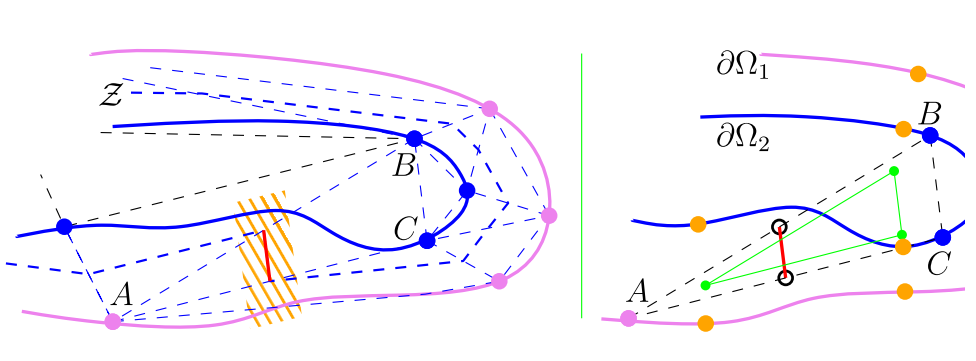
\includegraphics[width=12cm]{3}
	\caption[Misoriented element]
        {Misoriented element. Left: The zero-set of $\bigtriangleup ABC$ (red) has an in-correct normal. Right: The piecewise-linear function defined on $\bigtriangleup ABC$ should classify well the samples of $\mathcal{S}$, and the sample points in $\partial \Omega$ that are nearest to the vertices of a shrunk copy of $\mathtt{t}$ (in orange, not satisfied in this case).}
 	\centering
\end{figure}
\par To solve the first problem, we enforce the constraint let $f(\mathtt{s}) < 1 - \alpha$, and add an upper bound of $\alpha / \sigma$ on the Lipschitz constant of the piecewise-linear function to ensure that the zero-set does not cross $\partial \Omega$.  Noticing that  the Lipschitz constant $c=2/h$ (h is the height of the tetrahedron as illustrate in Figure 4), so $2/h < \alpha / \sigma$, and a tetrahedron between $\partial \Omega_1$ and $\partial \Omega_2$ with $h \le 2\sigma / \alpha$ is a bad tetrahedron. $\alpha$ is set to 0.2.
\begin{figure}[H]
 	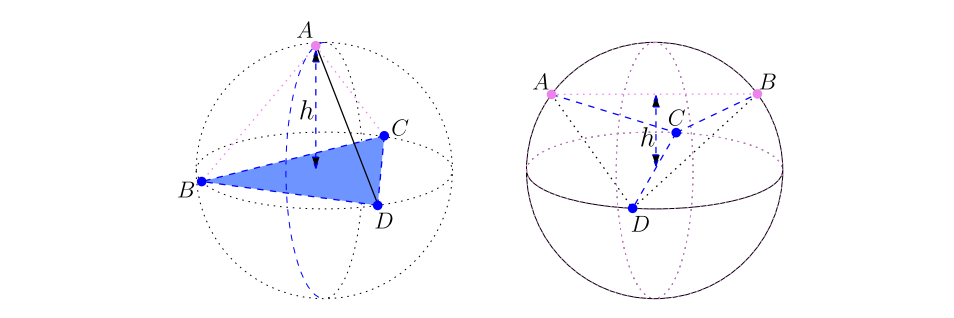
\includegraphics[width=12cm]{4}
	\caption[Height]
        {Height of a tetrahedron.}
 	\centering
\end{figure}
\par To solve the second problem, the piecewise-linear function defined by each tetrahedron $\mathtt{t}$ classifies well the samples of  $\mathtt{S}$ on both the points of $\partial \Omega$. But can't classifiy the sample points in $\partial \Omega$ that are nearest to the vertices of a shrunk copy of $\mathtt{t}$, then $\mathtt{t}$ is a bad tetrahedron. The size of this shrunk copy is set to 0.7.
\par So our algorithm procedure is:
\begin{description}
 \item[1.] Adding the sample point in  $\mathtt{S}$ withing the maximum error, until $\epsilon(\mathtt{s}) < 1- \alpha$.
 \item[2.] Adding the sample point nearest to the circumcenter of a bad tetrahedron.
\end{description}
The Figure 5 illustrates a refinment of 2D case.
\begin{figure}[H]
 	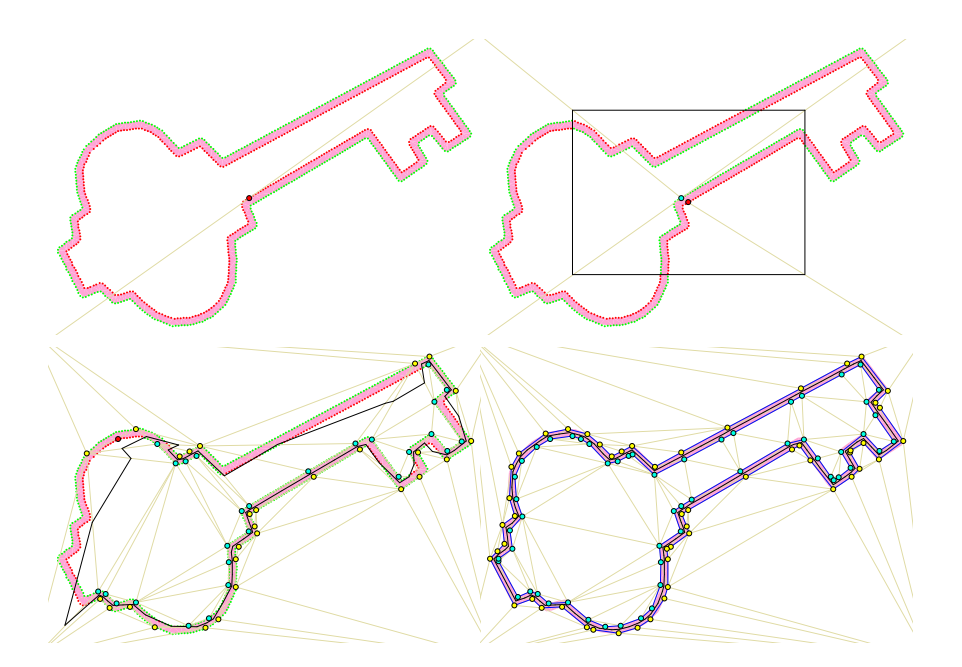
\includegraphics[width=12cm]{5}
	\caption[Refinment of 2D case]
        {Refinement of $\tau$ . Top: initial triangulation and one point inserted(\emph{here haven't draw the four conner points which construct the loose bounding rectangle}). Bottom: more points inserted, and
complete classification of samples. The zero-set is depicted with black solid edges. Samples classified as good are depicted in green, and in red otherwise. A point to be inserted at the next iteration is depicted in red. Upon termination the edges of $\partial \Gamma$ are depicted in blue.}
 	\centering
\end{figure}
\section{Simplification}
\subsection{Overview}
In this step our goal is to reduce the complexity of the zero-set $\mathcal{Z}$ via the decimation of $\tau$. We peform the decimation by flowing steps:
\begin{description}
  \item[1.] Collapse edges of $\partial \Gamma$.
  \item[2.] Mutualtessllation of $\mathcal{Z}$ into $\tau$.
  \item[3.] Collapse edges of $\mathcal{Z}$.
  \item[4.] Collapse all possibile edges.
\end{description}
\subsection{collapse edges of $\partial \Gamma$}
Define the an edge PQ collapse into a target point $\mathtt{T}$ from $\mathtt{S}$, We have conditions as flows:
\begin{itemize}
  \item Keep a valid triangulation $\tau$, or equivalently merge two points one time. See Figure 6  (common condition)
  \item Kernel area $K_{\tau}(PQ)$ of one ring edge PQ is not empty, as T must locate into that area, which makes one sample point only in one tetrahedron(the tetrahedron not intersect). See Figure 7. (common condition)
  \item Keep $\epsilon(s) < 1-\alpha$.
\end{itemize}
\begin{figure}[H]
 	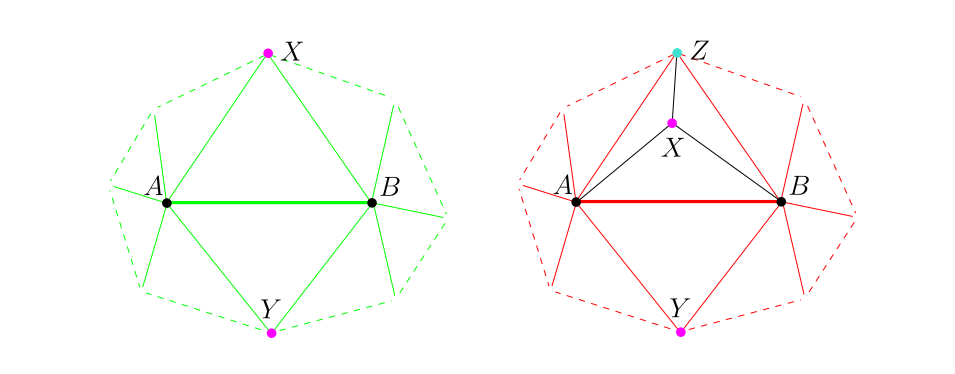
\includegraphics[width=12cm]{6}
	\caption[Link condition in 2D]
        {Link condition in 2D. Left: the edge AB is collapsible as
$Lk(A) \cap Lk(B) = Lk(AB)$. Right: the edge AB is not collapsible as $Lk(A) \cap Lk(B) \ne Lk(AB)$.}
 	\centering
\end{figure}
\begin{figure}[H]
 	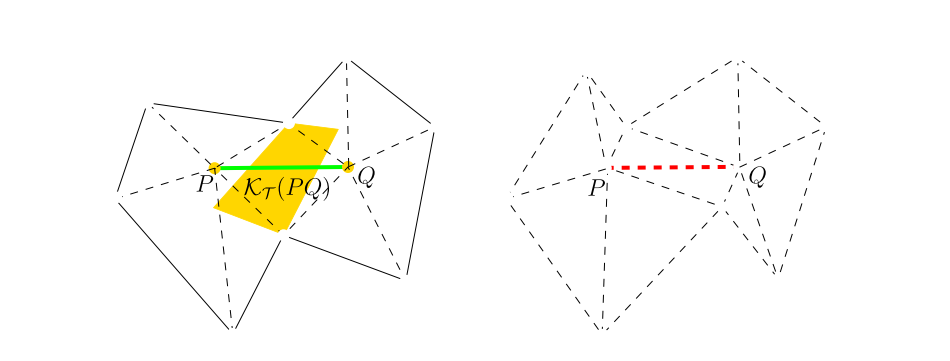
\includegraphics[width=12cm]{7}
	\caption[Kernel area]
        {2D中 $K_{\tau}(PQ)$ 是以PQ一环邻域的多边形的每一条边所对应的直线内侧的区域的$\cap$.。3D中 $K_{\tau}(PQ)$是以PQ为一环邻域的四面体所构成的多面体的各个面所对应的平面内侧的区域的$\cap$。}
 	\centering
\end{figure}
\par For the third condition, as we can see the collapse of edge PQ only affect the function value of the sample points of $\mathtt{S}$ in the one ring area of PQ, we define it by $\mathtt{W}$. So we just need to guarantee $\epsilon(\mathtt{s}) < 1-\alpha,  \mathtt{s \in W}$. To avoid exhaustive search, we discard the sample points leading to errors in the classification of $\mathtt{S}$, as located in invalid regions, denoted $\Psi$. We assume an edge of $\partial \Gamma$ PQ is collapsed into the target point T, and $\bigtriangleup ABT$ is a triangle in $\tau$ after the edge collapse. We solve this by two case discussion. See Figure 8 for reference.
\par Point AB and  point T  are in two different boundary respectively. If AB are on the inner boundary of $\partial \Gamma$, then for each point $E \in W$ we can construct a line $\mathtt{n} \parallel AB$, and a line $\mathtt{m} \parallel AB$ let $dis_{m \to n}/dis_{n \to AB} = \alpha/(2-\alpha)$, as we know $f(E) \ge 1-\alpha$. If T is located in the invalid area $\Psi$ (gray) then the classification of E is not preserved.  Similarly if AB are on the outer boundary. See Figure 8 left subfigure.
\par Point AT and point B are in two different boundary respectively. If BT is in outer boundary, and A is on inner boundary, find the point Y in AB where $\parallel BY \parallel / \parallel YA \parallel = \alpha/(2-\alpha)$, and $\mathtt{m} \parallel YE$ is a line cross B. Then we can get the invalid area $\Psi$ (gray) like the first case. See Figure 8 right subfigure.
\begin{figure}[H]
  \begin{subfigure}[b]{0.5\textwidth}
 	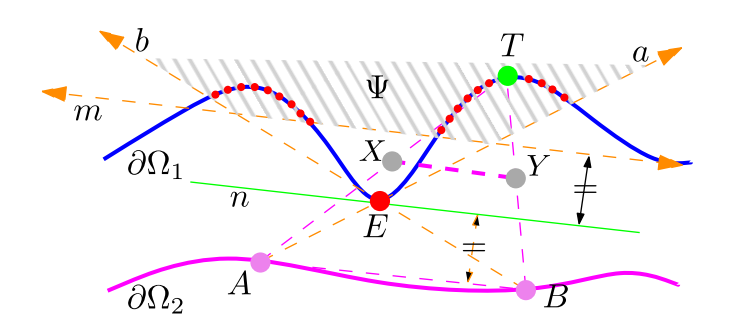
\includegraphics[width=\textwidth]{8}
        \caption[case 1]{case 1, a,b is let E in the $\bigtriangleup ABT$.}
  \end{subfigure}
  \begin{subfigure}[b]{0.5\textwidth}
      	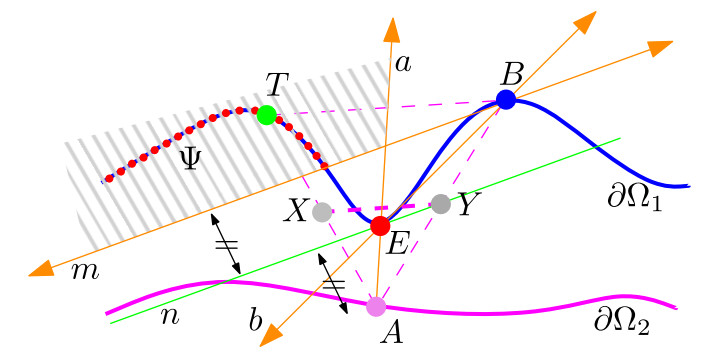
\includegraphics[width=6cm]{9}
        \caption[case 2]{case 2m a left E in the $\bigtriangleup ABT$}
   \end{subfigure}
  \caption[Edge Collapse] {Two case as discripted by above, in the paper the constraint $\epsilon(s) < 1$, I think its a mistake, it should be $\epsilon(s) <1-\alpha$.}
\end{figure}
\subsection{Mutualtessllation of $\mathcal{Z}$ into $\tau$}
Paper did not elaborate. See Figure 10.
\begin{figure}[H]
 	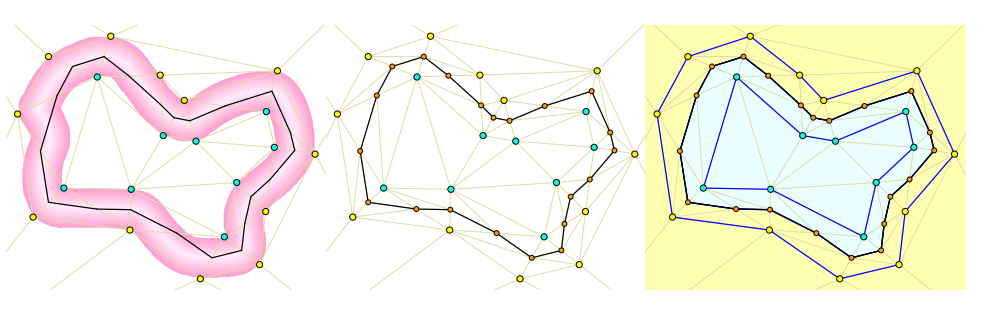
\includegraphics[width=\textwidth]{10}
	\caption[mt]
        {Mutual tessellation. Left: before mutual tessellation. Middle: after mutual tessellation. Right: classification of tetrahedra in accordance to $\partial \Omega$. The edges of $\mathcal{Z}$ and $\partial \Gamma$ are depicted with solid black and blue lines, respectively.}
 	\centering
\end{figure}
\subsection{Collapse edges of $\mathcal{Z}$}
With to common condition as above, and a different third condition: after edge collapse, the zero-set surface can't corss $\partial \Omega$. See Figure 11.
\begin{figure}[H]
 	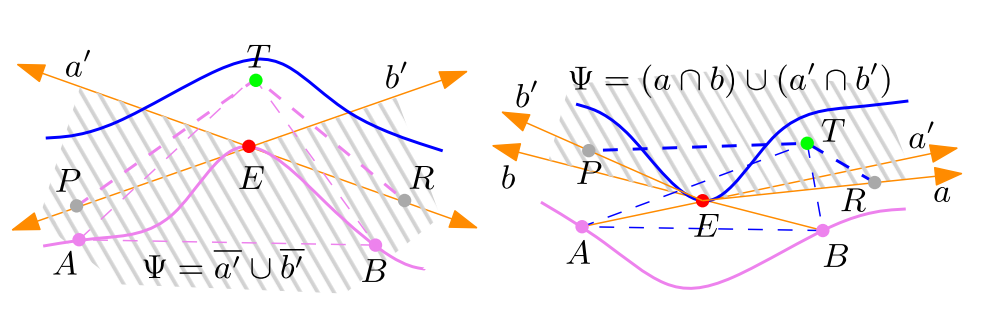
\includegraphics[width=\textwidth]{11}
	\caption[Edge Collapse of Z]
        {Invalid region. Assume an edge of $\mathcal{Z}$ is collapsed into the target point T (PTR represents the zero-set after collapse). The intersection of the two half-spaces delineated by a and b represents the locus of T which keeps E within $\bigtriangleup ABT$. Lines a and b represent the extreme zero-set originating from E that preserves the classification of point E. If $E \in \Psi$(gray), the classification of E is not preserved.}
 	\centering
\end{figure}

\subsection{Collapse all possibile edges}
In fact in this step we perform edge collapse between $\partial \Gamma$ and $\mathcal{Z}$, under the two common conditions. Collapsing an edge between a vertex of $\Gamma$ and a vertex of $\mathcal{Z}$ tends to increase the area of the one-ring of PQ  and hence increases the probability that an edge of $\mathcal{Z}$ is collapsible.
%% \begin{figure}[H]
%% 	\onecolumn
%% 	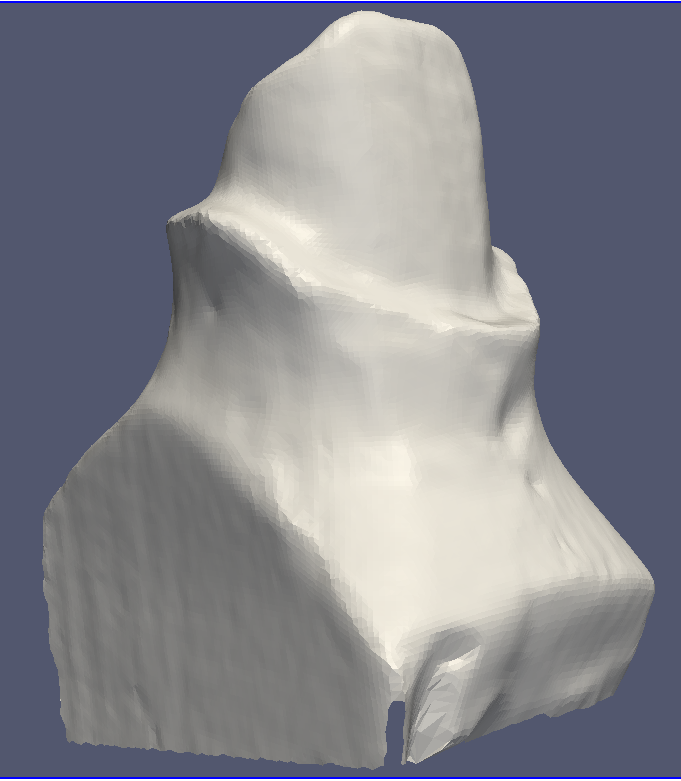
\includegraphics[width=6cm]{our_basic}
%% 	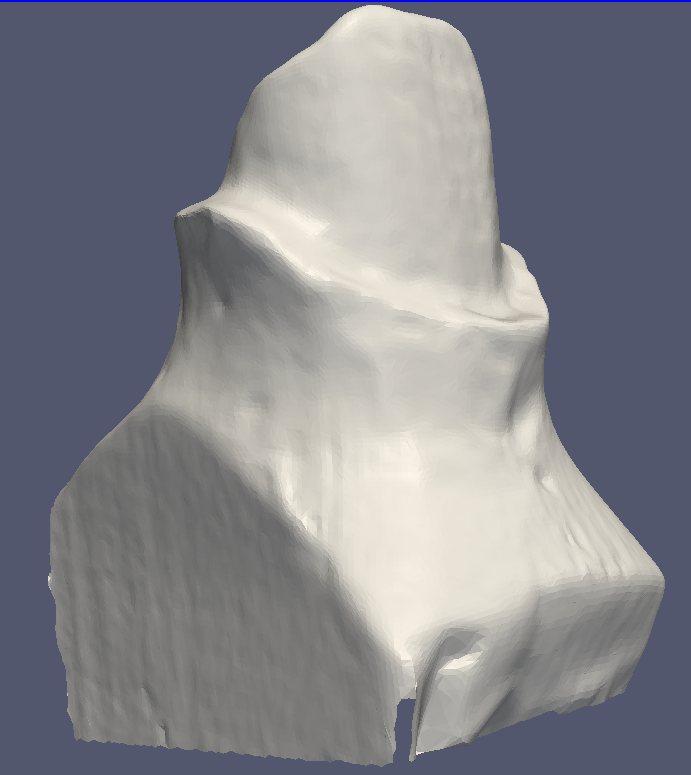
\includegraphics[width=6cm]{smooth_0}
%% 	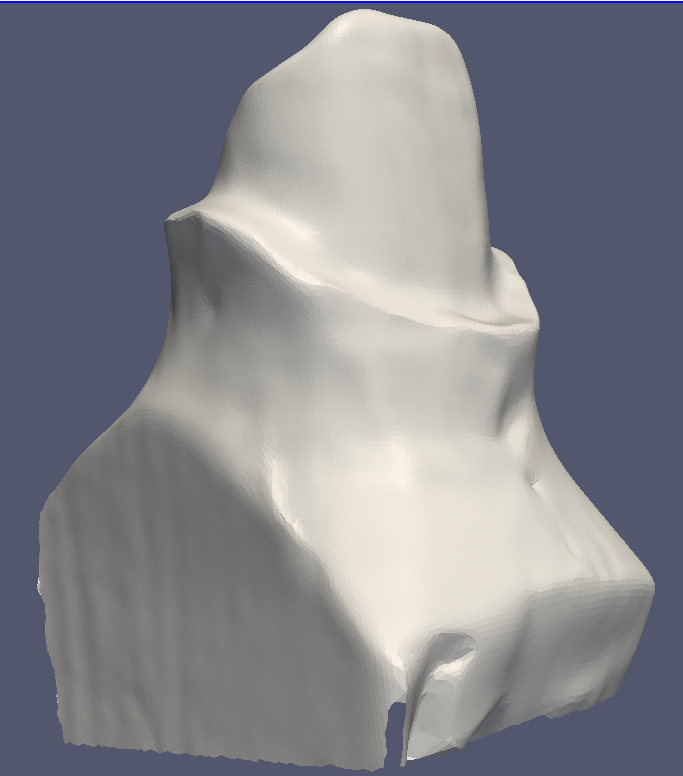
\includegraphics[width=6cm]{smooth_1}
%% 	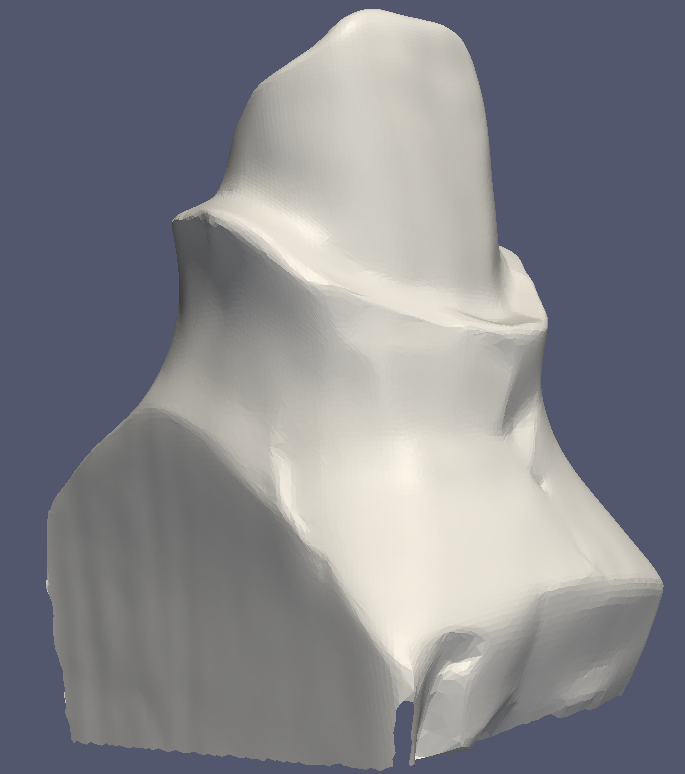
\includegraphics[width=6cm]{smooth_2}
%% 	\caption[效果对比]
%% 	{Atos不同程度光顺与标准双边滤波(3次迭代,边的一环邻域)效果对比,左上角为标准双边滤波效果,另外为geo inspect取不同滤波半径的结果,滤波半径依次扩大.}
%% 	\centering
%% \end{figure}

\end{document}
